\documentclass{beamer}
\usepackage{latexsym}
\usepackage{amssymb}
\usepackage{amsbsy}
\usepackage{alltt}
\usepackage{tikz}
\usepackage{stmaryrd}

\newcommand{\imp}{\Rightarrow}
\newcommand{\etal}{\textit{et. al}}
\newcommand{\adhoc}{\textit{ad hoc}}
\newcommand{\ie}{\textit{i.e.}}
\newcommand{\etc}{\textit{etc}}
\newcommand{\eg}{\textit{e.g.}}
\newcommand{\konst}[1]{\ensuremath{\mbox{\bf{#1}}}}
\newcommand{\nil}{\konst{[\,]}}
\newcommand{\cons}[2]{{#1}\boldsymbol{:}\boldsymbol{:}{#2}}
\newcommand{\hollamb}{\boldsymbol{\lambda}}
\newcommand{\itelse}[3]{\mbox{$\mbox{\tt if}\ {#1}\ \mbox{\tt then}\ {#2}\
    \mbox{\tt else}\ {#3}$}}
\newcommand{\set}[1]{\{ {#1} \}}
\newcommand{\Lang}[1]{\ensuremath{{\cal L}({#1})}}
\newcommand{\inbox}[1] {\begin{center}
                         \framebox{\parbox{0.984\textwidth}{#1}}
                         \end{center}}
\newcommand{\den}[1]{%
  \ensuremath{%
    \left\llbracket{#1}
    \right\rrbracket}}

% for backslashes in alltt environments
\newcommand{\bs}{\texttt{\symbol{92}}}

\usetikzlibrary{shapes}


\begin{document}

\begin{frame}\frametitle{Son of SPLAT}

\hspace{50mm}
{\small
\begin{tabular}{l}
Konrad Slind \\ Collins Aerospace \\ Trusted Systems Group Presentation \\ April 7 2020
\end{tabular}
}

\end{frame}

\begin{frame}\frametitle{Overview}

\konst{SPLAT}\footnote{SPLAT = \textit{Semantic Properties for
    Language and Automata Theory}} is a plugin to the Collins
"Architecture-Level Designer Workbench" being designed and implemented
by Isaac.

\vspace{10mm}

\konst{SPLAT} provides support for adding filters between components
in order to prevent reception of badly formed or malicious messages.

\vspace{10mm}

There is ongoing work to provide similar support for runtime monitoring (\konst{SPLAT-MON})

\end{frame}

\begin{frame}\frametitle{Semantics-based tool generation}

A way to think about \konst{SPLAT} is that a collection of useful
tools are generated from a central notation that has a formal semantic
definition (regexps and regular languages at present).

\vspace*{10mm}

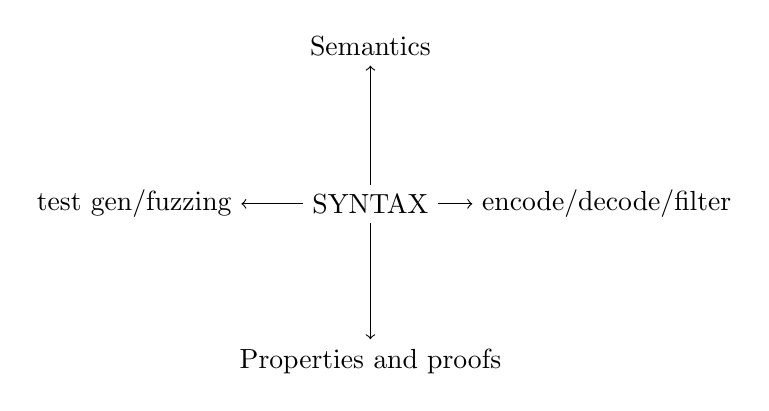
\begin{tikzpicture}[auto]
\node (SYNTAX) at (0,0) {SYNTAX};
\node (TEST) at (-3,0) {test gen/fuzzing};
\node (SEM) at (0,2) {Semantics};
\node (PROP) at (0,-2) {Properties and proofs};
\node (IMPL) at (3,0) {encode/decode/filter};
\draw [->] (SYNTAX) to (TEST);
\draw [->] (SYNTAX) to (SEM);
\draw [->] (SYNTAX) to (PROP);
\draw [->] (SYNTAX) to (IMPL);
\end{tikzpicture}
\end{frame}

\begin{frame}\frametitle{\konst{SPLAT} functionality in CASE}

\begin{itemize}
  \item Input: an AADL architecture annotated with filter specifications
\vspace*{5mm}
  \item Output: a logical theory containing the following elements for
    each filter specified in the architecture:

\begin{itemize}

  \item[-] declaration of the record and enumeration type(s) corresponding to
    the relevant AADL connection type

  \item[-] definition(s) of the wellformedness of the filter input (scraped from AGREE spec)

  \item[-] a table-driven DFA that renders a pass-fail verdict on messages,
    allowing only wellformed messages to pass

  \item[-] encoder and decoder mapping between records and the message format

  \item[-] theorems showing the correctness of the DFA.

\end{itemize}
\end{itemize}
\end{frame}

\begin{frame}\frametitle{Picture}
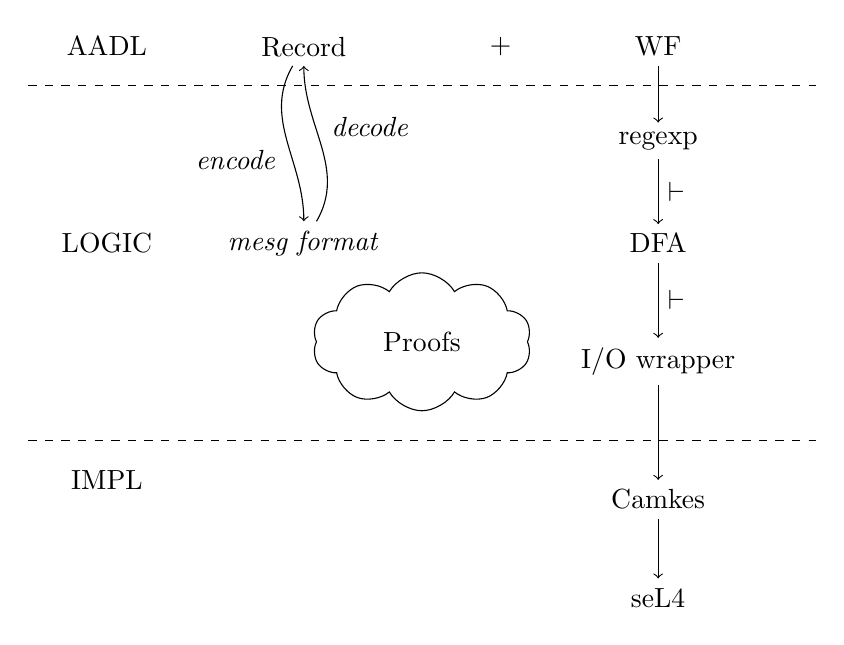
\begin{tikzpicture}[auto]
\node (AADL) at (1,0) {AADL};
\node (RECD) at (3.5,0) {Record};
\node () at (6,0) {+};
\node (WF) at (8,0) {WF};
\node (LOGIC) at (1,-2.5) {LOGIC};
\node (MESG) at (3.5,-2.5) {\textit{mesg format}};
\node (REGEXP) at (8,-1.2) {regexp};
\node (DFA) at (8,-2.5) {DFA};
\node (IOWRAP) at (8,-4) {I/O wrapper};
\node (CLOUD) [cloud, draw,cloud puffs=10,cloud puff arc=120, aspect=2, inner ysep=1em] at (5,-3.75) {Proofs};
\node (IMPL) at (1,-5.5) {IMPL};
\node (CAMKES) at (8,-5.75) {Camkes};
\node (SEL4) at (8,-7) {seL4};
\draw [dashed] (0,-0.5) -- (10,-0.5);
\draw [dashed] (0,-5) -- (10,-5);
\draw [->] (WF) to (REGEXP);
\draw [->] (REGEXP) to node{$\vdash$} (DFA);
\draw [->] (DFA) to node{$\vdash$} (IOWRAP);
\draw [->] (IOWRAP) to (CAMKES);
\draw [->] (CAMKES) to (SEL4);
\draw [->] (RECD) to [out=-120,in=north] node[swap]{\textit{encode}}(MESG);
\draw [->] (MESG) to [out=60,in=south] node[swap]{\textit{decode}}(RECD);
\end{tikzpicture}

\end{frame}


\begin{frame}\frametitle{Limitations}

The \konst{SPLAT} approach attempts to reap the benefits of
approximately 50 years of formal language technology development. We
have had some success.

\vspace*{5mm}

BUT!

\begin{itemize}
 \item Many useful message formats not able to be captured by regexps
   and DFAs (or even grammars). So the usual tools won't work.
\vspace*{5mm}
 \item Inter-field relationships expressible by standard formal language technology
\vspace*{5mm}
 \item Underlying technology for DFA generation (Brzozowski derivatives) is hard to make efficient
\end{itemize}

\end{frame}


\begin{frame}\frametitle{\konst{SPLAT++}}

The goal is to have the same nice picture except with a more
expressive formalism in the middle of things. But what can it be?

\vspace*{10mm}

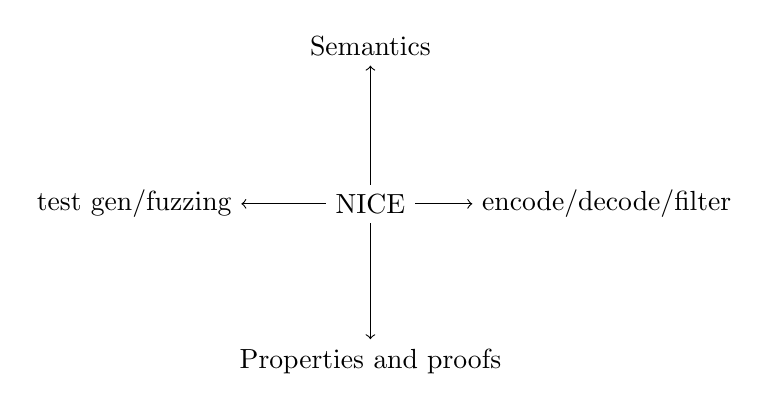
\begin{tikzpicture}[auto]
\node (SYNTAX) at (0,0) {NICE};
\node (TEST) at (-3,0) {test gen/fuzzing};
\node (SEM) at (0,2) {Semantics};
\node (PROP) at (0,-2) {Properties and proofs};
\node (IMPL) at (3,0) {encode/decode/filter};
\draw [->] (SYNTAX) to (TEST);
\draw [->] (SYNTAX) to (SEM);
\draw [->] (SYNTAX) to (PROP);
\draw [->] (SYNTAX) to (IMPL);
\end{tikzpicture}
\end{frame}

\begin{frame}\frametitle{Problems!}

\begin{itemize}
\item Many message formats fall outside the realm of common formal
  language techniques. We call these \emph{self-describing} formats
  since information in fields of the message influences the structure
  of the message.

\item For example, variable-length fields are a self-describing
  feature. Alas, can't be handled by regular or context-free techniques.

\item Context-sensitive languages can---\emph{in principle}---specify such
  information, but there are few (if any) tools supporting CSLs.

\item Another possibility would be to use so-called parser combinators in
order to quickly stitch together a parser; it's possible the
combinators could be instrumented to include contextual information.

\item In general, we need to be able to lex/parse/filter in a setting
  where information already encountered in the message is used to
  determine subsequent lexing/parsing/filtering steps.

\end{itemize}
\end{frame}

\begin{frame}\frametitle{Contiguity types}

\begin{itemize}

\item The characteristic feature of a message is that its fields are
  \emph{contiguous} \ie, placed side-by-side.

\vspace*{5mm}

\item Let's try to say where the fields of a message \emph{come from}
  in terms of PL datastructures.

\[
\begin{array}{rcl}
 \mathit{base} & = & \konst{bool} \mid \konst{char} \mid \konst{u8} \mid
 \konst{u16} \mid \konst{u32} \mid \konst{u64}  \mid \konst{i16} \mid
 \konst{i32} \mid \konst{i64} \mid \cdots \\
 \tau & = & \mathit{base} \\
      & \mid & \konst{Recd}\; (f_1 : \tau_1) \ldots (f_n : \tau_n) \\
      & \mid & \konst{Array}\; \tau \; \mathit{exp} \\
      & \mid & \konst{Union}\; (\mathit{bexp}_1 : \tau_1) \ldots (\mathit{bexp}_n : \tau_n)
\end{array}
\]

\end{itemize}

\end{frame}

\begin{frame}\frametitle{Contiguity types (contd)}

Given any such type, \ie, combination of records, arrays, and unions
over base types, one knows how to lay the corresponding datastructure
out in memory, and also how to parse a patch of memory into such a
datastructure.

\vspace*{5mm}

The trick is how to accumulate and exploit the information in self-describing messages.

\vspace*{5mm}

This is what the expression language does. It provides syntax to
reference previously seen fields or array elements.

\vspace*{5mm}

\end{frame}


\begin{frame}[fragile]\frametitle{Example}

A straightforward record where each field is of a statically known size.

\begin{verbatim}
  {A : u8
   B : {name : char [13]
        cell : i32}
   C : bool
  }
\end{verbatim}
\end{frame}

\begin{frame}[fragile]\frametitle{Example}

Variable-sized strings

\begin{verbatim}
  {len : u16
   elts : char [len]
  }
\end{verbatim}
\end{frame}


\begin{frame}[fragile]\frametitle{Example}

Contrived example showing resolution of multiple similarly named fields.

\begin{verbatim}
  {len : u16
   A : {len : u16
        elts : u16[len]
       }
   B : char [A.len * len]
   C : i32 [A.elts[0]]
  }
\end{verbatim}

\end{frame}

\begin{frame}[fragile,allowframebreaks]\frametitle{Example: MAC header in 802-11}

First we need an enumerated type (enumerated
types can be used in contiguity types)

\begin{verbatim}
 enum Frame = [("Management",0),
               ("Control",   1),
               ("Data",      2),
               ("Reserved",  3)]
\end{verbatim}

\vspace*{5mm}

The actual MAC header description is in terms of bits while our
current implementation is for bytes. We use the $\konst{Raw}(n)$
construct to break off a chunk of $n$ bytes. (Changing to bits would
require very little effort.)


\begin{verbatim}
   {protocol  : Raw(2)
    type      : Frame
    subType   : Raw(4)
    toDS      : Raw(1)
    fromDS    : Raw(1)
    moreFrag  : Raw(1)
    retry     : Raw(1)
    powerMgmt : Raw(1)
    moreData  : Raw(1)
    wep       : Raw(1)
    order     : Raw(1)
    duration  : Raw(16)
    tails     : Union {
     (type = Frame'Data)
          --> {address1   : Raw(48)
               address2   : Raw(48)
               address3   : Raw(48)
               fragNumber : Raw(4)
               seqNumber  : Raw(12)
               address4   : Raw(48)
              }
     (type = Frame'Control and subType = 11)
          --> {receiver    : Raw(48)
               transmitter : Raw(48)
              }
     (type = Frame'Control and subType = 12)
          --> {receiver : Raw(48)
              }
     }
    }
\end{verbatim}

\end{frame}

\begin{frame}[fragile,allowframebreaks]\frametitle{Example: uxAS AirVehicleState}

\begin{verbatim}
AirVehicleState =
   {EntityState   : EntityState
    Airspeed      : Float
    VerticalSpeed : Float
    WindSpeed     : Float
    WindDirection : Float
   }
\end{verbatim}

\noindent where

\begin{verbatim}
EntityState =
   {ID : i64
      ...
    Location :
      {Latitude : Double
       Longitude : Double
       Altitude : Float
       AltitudeType : AltitudeType
      }
     ...
    PayloadStateListLen : u16
    PayloadStateList :
     {PayloadID : i64
      ParametersLen : u16
      Parameters : KeyValuePair [ParametersLen]
      } [PayloadStateListLen]
     ...
    InfoLen : u16
    Info : KeyValuePair [InfoLen]
    }
\end{verbatim}

\noindent and (among many other things)
\begin{verbatim}
KeyValuePair =
   {key   : String
    value : String
   }
\end{verbatim}

So PayloadStateList is a variable-length array of records, each of
which has a variable-length array of KeyValuePairs, each of which is a
pair of variable-length strings. Monstrous!
\end{frame}

\begin{frame}\frametitle{Parser generation}

The good news is that message lexers and parsers can be automatically
generated from contiguity types. The parser generator is surprisingly
simple (about 300 lines of SML).

\vspace*{5mm}

The secret to parsing with contiguity types is that the type is
traversed in top-down, left-to-right order, and each step of traversal
advances through the string and adds a new piece of information to the
parsing context.

\vspace*{5mm}

In a sense, the tree that is the contiguity type is incrementally
being flattened out and superimposed on to the string being parsed.

\vspace*{3mm}

The contiguity type describes a C-style \emph{l-value}. Traversing the
type visits (and determines the value of) every location that could be
mentioned in later array indices or union discriminators.

\end{frame}

\begin{frame}\frametitle{\konst{SPLAT++}}

I think the nice picture is achievable with contiguity types. The
upshot: if you can describe your message format with a contiguity
type, then a parser (and soon, filters) can be automatically generated
for you. It should also be the case that formal correctness proofs are
also generated.

\vspace*{10mm}

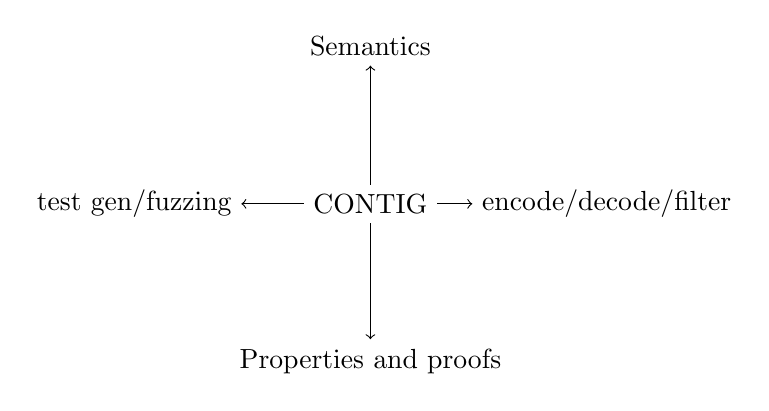
\begin{tikzpicture}[auto]
\node (SYNTAX) at (0,0) {CONTIG};
\node (TEST) at (-3,0) {test gen/fuzzing};
\node (SEM) at (0,2) {Semantics};
\node (PROP) at (0,-2) {Properties and proofs};
\node (IMPL) at (3,0) {encode/decode/filter};
\draw [->] (SYNTAX) to (TEST);
\draw [->] (SYNTAX) to (SEM);
\draw [->] (SYNTAX) to (PROP);
\draw [->] (SYNTAX) to (IMPL);
\end{tikzpicture}
\end{frame}

\begin{frame}\frametitle{Current status and future work}

\begin{itemize}
\item Copy-free parser generator working
\item Formal semantics (in progress)
\item Correctness proof for parser generator
\item Relationship with encode-decode proofs
\item Push formal parsing engine to CakeML, compile, and test
\item Test on real uxAS messages
\item Start thinking about CASE Phase III messages (ADS-B for example)
\item Develop property specification support (lvals help)
\item Instantiate test-gen functionality
\item Get implementations going in other languages (ACL2, Slang, C, ...)
\item Discuss relationship with Luke Ryon's \konst{SALP} language
\end{itemize}
\end{frame}


\end{document}
